% Created 2025-10-06 Mon 13:43
% Intended LaTeX compiler: lualatex
\documentclass[a4paper,12pt]{article}
\usepackage{amsmath}
\usepackage{fontspec}
\usepackage{graphicx}
\usepackage{longtable}
\usepackage{wrapfig}
\usepackage{rotating}
\usepackage[normalem]{ulem}
\usepackage{capt-of}
\usepackage{hyperref}
\usepackage{luacode}
\usepackage[english, french]{babel}
\usepackage{microtype}
\usepackage[autolanguage]{numprint}
\npthousandsep{~}
\usepackage{fontspec}
\usepackage{ulem}
\usepackage{soul}
\setmainfont{Source Serif 4}[Path=/home/anthea/org/fonts/Source_Serif_4/static/, UprightFont=SourceSerif4-Regular.ttf, ItalicFont=SourceSerif4-Italic.ttf, BoldFont=SourceSerif4-Bold.ttf, BoldItalicFont=SourceSerif4-BoldItalic.ttf]
\setsansfont{Source Sans 3}[Path=/home/anthea/org/fonts/Source_Sans_3/static/, UprightFont=SourceSans3-Regular.ttf, ItalicFont=SourceSans3-Italic.ttf, BoldFont=SourceSans3-Bold.ttf, BoldItalicFont=SourceSans3-BoldItalic.ttf]
\setmonofont{Source Code Pro}[Path=/home/anthea/org/fonts/Source_Code_Pro/static/, UprightFont=SourceCodePro-Regular.ttf, ItalicFont=SourceCodePro-Italic.ttf, BoldFont=SourceCodePro-Bold.ttf, BoldItalicFont=SourceCodePro-BlackItalic.ttf]
\renewcommand{\familydefault}{\sfdefault}
\renewcommand{\tiny}{\small}
\renewcommand{\scriptsize}{\small}
\usepackage[usenames,dvipsnames,svgnames,table]{xcolor}
\definecolor{customgray}{HTML}{505050}
\usepackage[top=3.2cm, bottom=3.2cm, left=2.4cm, right=2.4cm]{geometry}
\usepackage{setspace,fancyhdr,indentfirst,lastpage,datetime,authblk,ifthen,etoolbox,titling}
\singlespacing
\pagestyle{fancy}
\fancyhf{}
\fancyfoot[C]{\thepage\ / \pageref{LastPage}}
\renewcommand{\headrulewidth}{0pt}
\setlength{\parindent}{0pt}
\setcounter{secnumdepth}{3}
\setlength{\columnsep}{0.8cm}
\setlength{\marginparwidth}{1.6cm}
\setcounter{page}{1}
\usepackage{csquotes}
\usepackage{array,booktabs,multirow,tabularx,colortbl,diagbox,makecell,ltablex,adjustbox,multicol}
\usepackage{enumitem}\setlist{nosep}\setlist[itemize]{leftmargin=*}
\usepackage[toc,page]{appendix}
\usepackage[nottoc]{tocbibind}
\newenvironment{keyword}{\begin{trivlist}\item[]{\bfseries Mots-clés :}}{\end{trivlist}}
\usepackage{graphicx,caption,wrapfig}
\usepackage[most,breakable,xparse,listings,skins]{tcolorbox}
\usepackage[colorinlistoftodos]{todonotes}
\usepackage{newfloat}
\DeclareFloatingEnvironment[fileext=lol,listname={\vspace{-2em}},name=Listing]{listing}
\captionsetup{format=plain,font=small,labelfont=bf}
\captionsetup[listing]{labelfont=bf,textfont=it}
\usepackage{fvextra,amsfonts,amssymb,amsmath,mathrsfs,mathtools,stmaryrd}
\usepackage{algorithm2e}
\usepackage{pgf,tikz,pgfplots,pgfplotstable,arydshln,subcaption,forest}
\pgfplotsset{compat=1.18}
\usepackage[acronym]{glossaries}
\makenoidxglossaries
\usepackage{url,orcidlink,hyperref}
\hypersetup{colorlinks=true, linkcolor=customgray, citecolor=customgray, urlcolor=customgray, pdfborder={0 0 0}, unicode=true}
\author{Laboratoire LAMIH-UMR CNRS 8201 Université Polytechnique Hauts-de-France, INSA, Valenciennes}
\date{\today}
\title{Développement du sujet de recherche}
\hypersetup{
 pdfauthor={Laboratoire LAMIH-UMR CNRS 8201 Université Polytechnique Hauts-de-France, INSA, Valenciennes},
 pdftitle={Développement du sujet de recherche},
 pdfkeywords={},
 pdfsubject={},
 pdfcreator={},
 pdflang={French}}
\usepackage[style=backend=biber,style=iso-numeric,citestyle=numeric-comp,doi=true,isbn=true,mincrossrefs=2,autocite=superscript]{biblatex}
\addbibresource{~/org/references.bib}
\begin{document}

\maketitle
\section{Titre de la thèse}
\label{sec:org1ed4088}

Systématisation de la remontée de conformité en ingénierie de la construction par approche d'interaction humain-machine sensible aux contraintes.

\begin{abstract}
Cette thèse vise à concevoir, réaliser et évaluer une interface utilisateur sensible aux contraintes pour améliorer la remontée de conformité en ingénierie de la construction, en se concentrant sur les systèmes électriques. Le projet s'articule autour de trois axes principaux : l'extraction dynamique des contraintes fonctionnelles et organisationnelles, l'amélioration de l'interaction humain-machine, et l'adoption de méthodologies agiles inspirées du génie logiciel. L'objectif est de créer un outil interactif permettant aux acteurs non spécialistes d'identifier et d'anticiper les infractions aux contraintes électriques dès la phase de conception. La recherche s'appuiera sur les concepts d'interface écologique et de réduction de la charge mentale. Le projet intégrera des approches de traitement du langage naturel et d'ontologies pour faciliter l'extraction et la gestion des contraintes. L'approche proposée permettra une vérification systématique et automatisée des contraintes tout au long du cycle de vie du projet, réduisant ainsi les risques d'erreurs. Les résultats de cette recherche pourraient contribuer à l'amélioration de la qualité, de la gestion des risques et de l'efficacité des projets de construction.
\end{abstract}

\begin{keyword}
Interaction humain-machine, interface utilisateur, interface écologique, contraintes, sensibilité aux contraintes, construction, énergie, électrotechnique, bâtiment.
\end{keyword}
\section{Contexte}
\label{sec:orgbe5ffe8}

L'industrie de la construction connaît une transformation profonde depuis les années 2000 avec l'émergence des outils de  (\protect\hyperlink{gls-1}{\label{gls-1-use-1}BIM}) et le cadre de travail qui en découle : le  (\protect\hyperlink{gls-2}{\label{gls-2-use-1}VDC}) \footnote{\protect\hyperlink{gls-2}{\label{gls-2-use-2}VDC}: Virtual Design and Construction, the use of integrated multi-disciplinary performance models of design-construction projects to support explicit and public business objectives \autocite{delsavioVirtualDesignConstruction2022a}.} \autocite{mohamedadelIntegrationBuildingInformation2022}.

L'adoption des standards et des bonnes pratiques liées au \protect\hyperlink{gls-1}{\label{gls-1-use-2}BIM} devait permettre d'augmenter l'efficacité lors des phases de conception et d'optimiser les phases d'exécution des projets de construction au prix d'une complexification des protocoles d'études \autocite{lindbladBIMImplementationOrganisational2015}. La réalisation des maquettes numériques, en se superposant aux métiers historiques liés à la construction pose le risque de favoriser ses propres objectifs plutôt que de se mettre au service des métiers historiques \autocite{lourauAnalyseInstitutionnelleQuestion1973}.

Cette évolution du contexte et des pratiques apporte un ensemble de contraintes additionnelles à un environnement déjà fortement régulé : en ingénierie de la construction, les corps d'état technique doivent en effet satisfaire de nombreuses contraintes. Celles-ci sont formalisées par les parties prenantes et par des institutions externes. Ces contraintes ont des sources diverses \autocite{artokiviniemiPREMISSRequirementsManagement2004} :
\begin{itemize}
\item des sources réglementaires : issues des normes et des textes de loi (code du travail, code des marché publiques, code de la construction\ldots{}),
\item des sources normatives : issues des recueils de bonne pratiques ou de référentiels standardisés (ISO 9001, NF C15-100, NF DTU\ldots{}),
\item des sources contextuelles : issues des spécifications propres à un projet (Cahier des charges, Spécifications Techniques, Contrat de prestation\ldots{}).
\end{itemize}

Le recensement des contraintes sur un projet donné est une tâche manuelle fastidieuse, chronophage et source d'erreurs. Des matrices de correspondance permettent d'indiquer au lecteur averti les documents qui contiendront la réponse à chacune des contraintes identifiées. Ce travail présente de nombreuses vulnérabilités telles que le risque d'erreur d'interprétation ou d'oubli, le manque d'ergonomie et le manque d'efficience. Après cette étape de modélisation, un ou plusieurs référents sont identifiés pour assurer le suivi de la prise en compte de ces contraintes. Ce suivi souffre d'un caractère non-exécutable, impliquant une exploration manuelle des corpus documentaires lors des opérations de vérifications et de contrôle. Les contraintes peuvent être classées selon trois natures :
\begin{itemize}
\item une nature technique : contraintes liées au respect de conditions et de règles d'un métier donné et définies dans les cahiers des charges et textes normatifs,
\item une nature fonctionnelle : contraintes liées à la réponse à un besoin de fonctionnement d'une installation et définies dans les cahiers des charges et textes normatifs,
\item une nature organisationnelle : contraintes de toutes autres natures et définies par les contrats, normes et lois.
\end{itemize}

\begin{figure}[htbp]
\centering
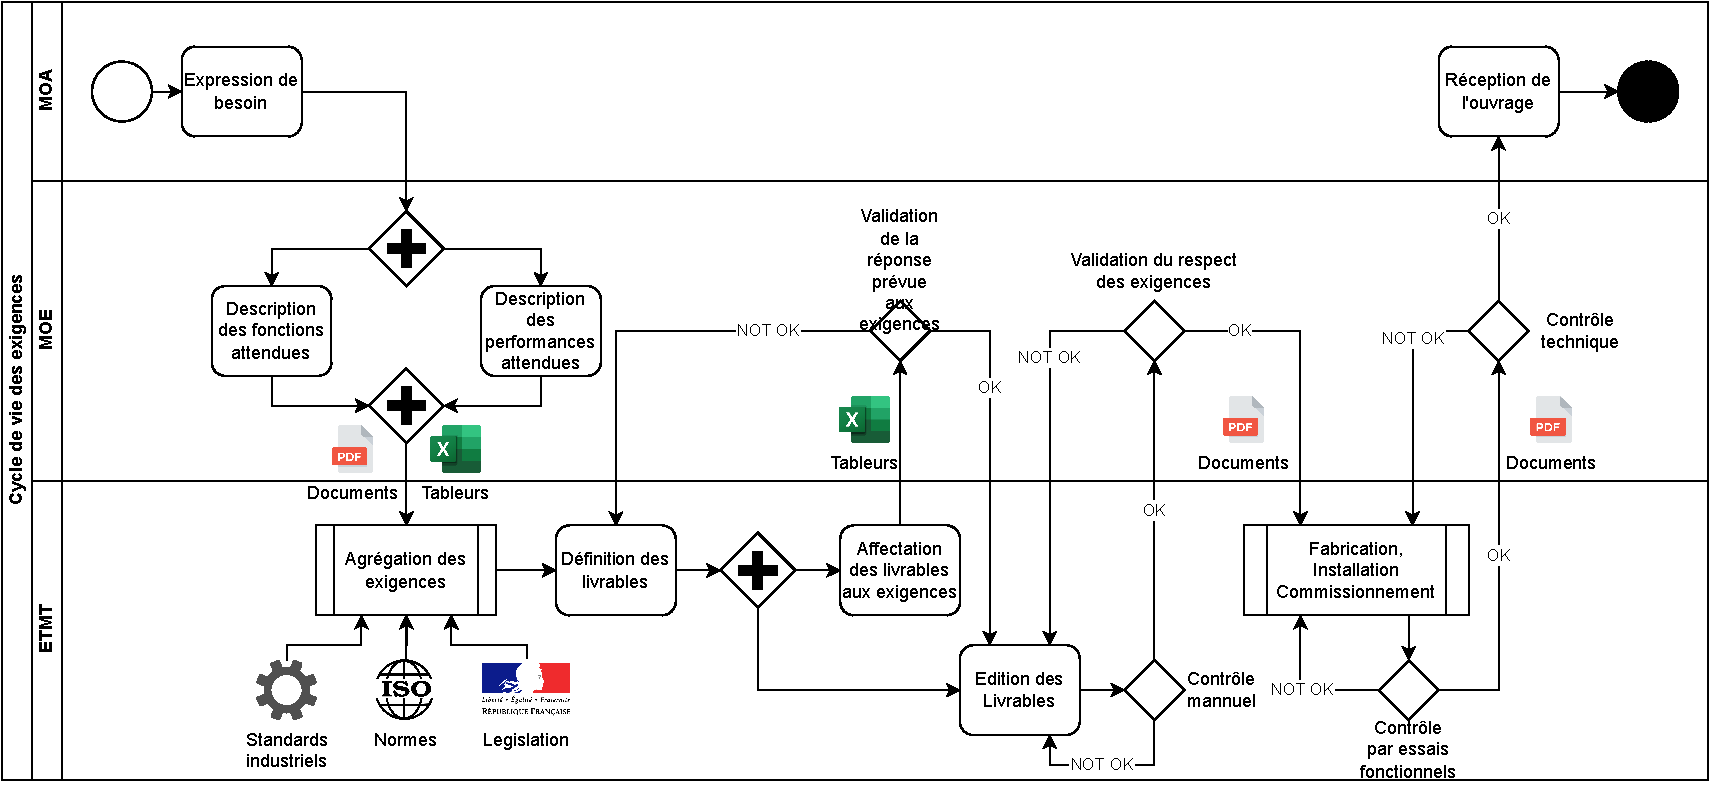
\includegraphics[width=.9\linewidth]{../svg/BPMN-LifeCycle-Exigences-init.pdf}
\caption{\label{fig:org53ca869}Macro-processus de traitement des contraintes durant un projet de construction.}
\end{figure}

Des protocoles et procédures sont mis en \{\oe\}uvre pour assurer la satisfaction de ces contraintes. La figure \ref{fig:org53ca869} présente le cycle de vie d'une contrainte exprimée par un client en schématisant sa précision par le maître d'\{\oe\}uvre et son intégration par l'entreprise générale.


La réalisation de notes de calculs, de simulations et de mesures physiques sont des exemples très représentatifs de systèmes de remontée de preuve adaptés aux contraintes techniques. Il n'existe cependant pas de système permettant une remontée de preuve d'un niveau qualitatif équivalent pour les contraintes fonctionnelles et organisationnelles. Ce périmètre est alors limité à l'apport en connaissance individuelle et repose entièrement sur un système de confiance pair-à-pair.

Les bâtiments contemporains sont parcourus par de nombreux réseaux électriques \footnote{Par abus de langage, nous considérons que les réseaux de fibres optiques font partie des réseaux électriques.} de différentes natures : signalisation, données, puissance. La diversité de ces réseaux implique une gestion complexe de contraintes diverses et sophistiquées : il peut s'agir d'interface avec le génie climatique sur l'alimentation d'équipements et des remontées de capteurs, de mise en \{\oe\}uvre de systèmes complexes de détection d'incendies reliés avec les sapeurs pompiers locaux ou encore la réalisation d'un réseau de surveillance et de sécurité assujetti à des dispositions de résilience informatique.

La multiplicité des domaines assujetti à ce corps d'état (gestion des réseaux électriques) augmente la quantité de clauses contractuelles ainsi que le corpus normatif et législatif à prendre en charge par les entreprises. Chaque sous-domaine requiert généralement l'expertise d'un spécialiste intervenant souvent en fin de cycle de conception.

Hélas, cette intervention peut advenir trop tardivement : une infraction de contrainte critique peut nécessiter le renvoi du projet en amont de la phase de conception et entraîner des coûts et des retards exorbitants. Ces catastrophes financières pourraient être évitées en proposant aux acteurs impliqués en amont du projet des outils interactifs faciles d'utilisation leur permettant d'identifier et de pallier, par anticipation, les infractions aux contraintes électriques qu'ils seraient susceptibles de commettre lors de la phase de conception. Pour ce faire, il s'agirait de rendre tangibles le fonctionnement et les contraintes des différents flux électriques, leurs interférences avec les équipements environnants ainsi que les autres réseaux et leurs contraintes sécuritaires et normatives par des retours visuels et textuels adaptés, respectant des critères d'utilisabilité (au sens de la norme ISO 9241-11:2018), et de surcroît cohérents avec la démarche cognitive inhérente à la phase de conception. Il serait ainsi possible de garantir le respect de ces contraintes à chaque modification du projet ou à intervalles réguliers à la manières des tests unitaires dont la pratique a été systématisée dans l'industrie du génie logiciel.
\section{Objet de la thèse}
\label{sec:org800d082}
Cette thèse s'inscrit dans une démarche de réponse à des enjeux majeurs rencontrés par les entreprises du secteur de la construction \autocite{guillouSegmentationDansEntreprises2003b} et notamment définis par les normes :
\begin{itemize}
\item Management de la qualité (ISO 9001),
\item Gestion des risques (X 50-117),
\item Maîtrise des coûts (X 50-137),
\item Maîtrise des délais (X 50-138),
\item Capitalisation sur l'expérience (X 50-190).
\end{itemize}

Cette thèse va tenter de proposer des pistes permettant de lever les verrous qui freinent l'exécution efficiente de la remontée de conformité en ingénierie de systèmes électriques. Pour ce faire, trois volets seront considérés.
\subsection{Volet d'ordre applicatif}
\label{sec:org4e7723e}
Différentes solutions de l'état de l'art seront étudiées afin de permettre l'extraction dynamique des contraintes fonctionnelles et organisationnelles. Les solutions étudiées seront tirées des domaines de traitement des langues naturelles appliqué aux corpus de textes réglementaires et législatifs ainsi que de l'état de l'art dans le domaine de la création et de l'échange d'ontologies appliquées au \protect\hyperlink{gls-1}{\label{gls-1-use-3}BIM}.
\subsection{Volet lié à l'interaction humain-machine}
\label{sec:orgddd701e}
Lorsqu'une contrainte est enfreinte, il est nécessaire de remonter à l'utilisateur non spécialiste la nature de l'infraction, sa ou ses causes et une ou plusieurs suggestions capables de lever l'infraction observée. Les solutions étudiées porteront sur les travaux liés à la conception d'Interfaces Utilisateur (UI) \autocite{Shneiderman2016}, la prise en compte de critères de l'eXpérience Utilisateur (UX) \autocite{Nogier2020} et la réduction de la charge mentale de travail \autocite{longoHumanMentalWorkload2022a,morayMentalWorkloadIts1979a} en situation d'interaction humain-machine. 
Parmi les approches étudiées, celle dite  d'interface écologique fera l'objet d'une attention particulière \autocite{vicenteEcologicalInterfaceDesign1992b,Burns2004}. Le but de telles interfaces est de rendre perceptivement évidentes à l'utilisateur les contraintes et les relations complexes constitutives de l'environnement de travail.
\subsection{Volet d'ordre méthodologique}
\label{sec:orgfb53348}
Les outils ne sont pas neutres \autocite{borremansGuideConvivialTools1979a}, ils permettent d'accompagner l'adoption de nouvelles méthodologies de travail. Les méthodes étudiées porteront notamment sur les pratiques agiles adoptées par l'industrie du génie logiciel et sur leur mise en place éventuelle dans le domaine de la construction. Nous étudierons en particulier comment la gestion itérative des modifications successives au projet (versioning) peut influencer l'organisation de la collaboration entre les différents acteurs d'un projet de construction.

Le processus présenté en figure \ref{fig:org53ca869} pourra évoluer vers une version allégée dont la figure \ref{fig:org73f51f3} propose un exemple.

\begin{figure}[htbp]
\centering
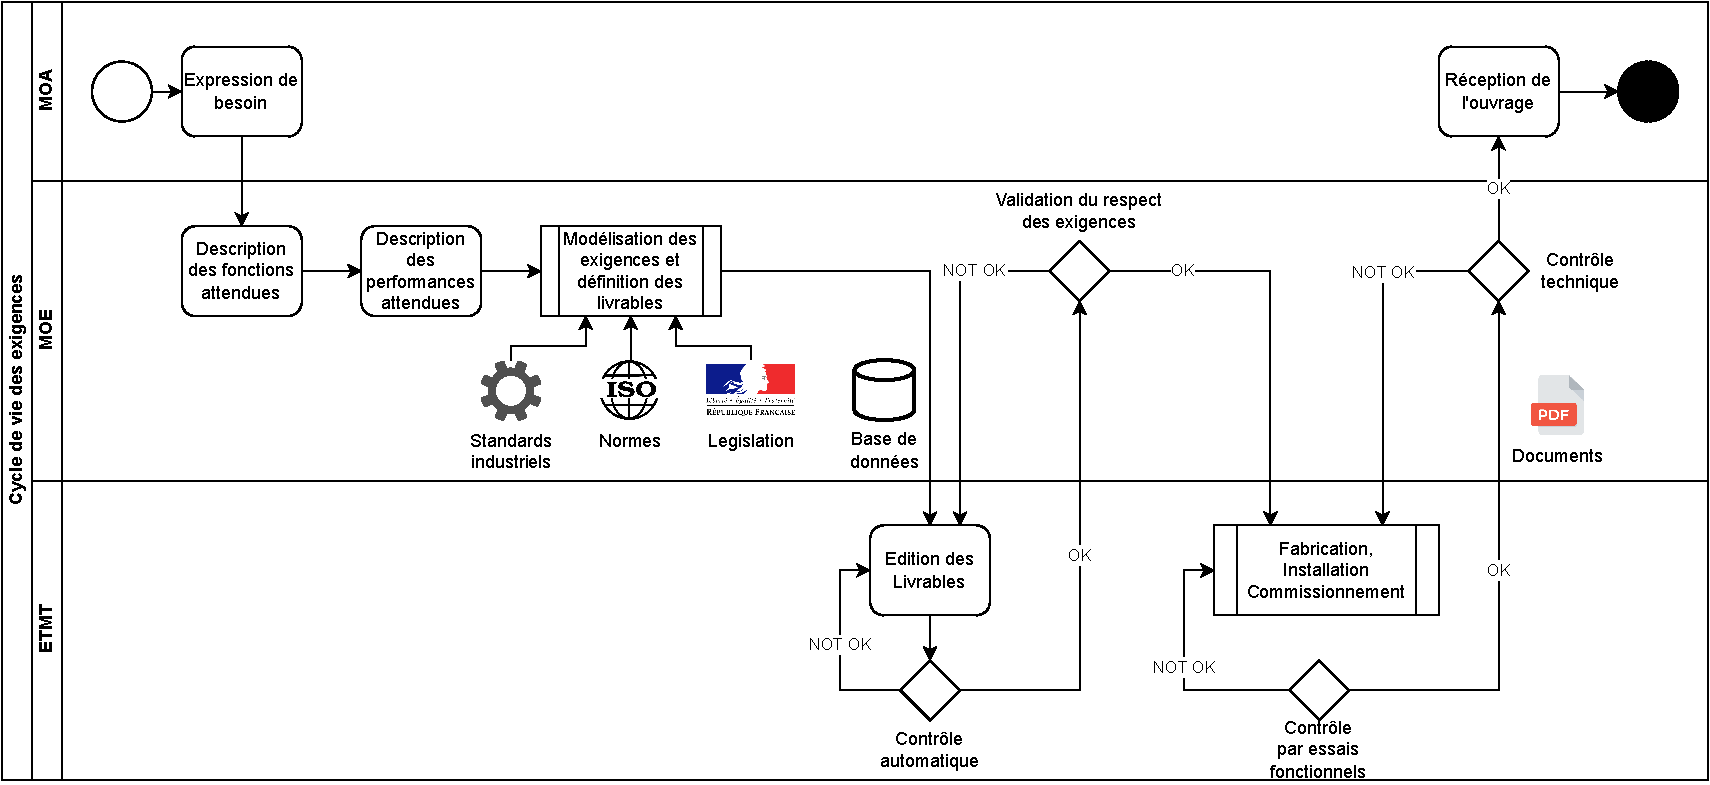
\includegraphics[width=.9\linewidth]{../svg/BPMN-LifeCycle-Exigences-target.pdf}
\caption{\label{fig:org73f51f3}Macro-processus de traitement des contraintes durant un projet de construction avec automatisation des vérifications d’études.}
\end{figure}
\section{Déroulement de la thèse}
\label{sec:orgfeae1cf}
La thèse se situe dans un projet CIFRE réunissant deux partenaires : le LAMIH-UMR CNRS 8201/UPHF (via son département Informatique, thème "Interaction et agents") et EIFFAGE ENERGIE SYSTEMES qui a une forte compétence, au sein de la direction I2S, sur la conception et l'intégration de réseaux hétérogènes dans des projets d'ouvrages d'art et d'infrastructure.


Date de démarrage souhaitée : Au plus tôt en 2025
\subsection{Phase 1 : Analyse de la problématique et étude bibliographique}
\label{sec:org990b053}
La première phase de cette étude se concentre sur l'exploration des interfaces humain-machine (IHM), en mettant l'accent sur  les approches permettant de contribuer à la sensibilité aux contraintes dans des espaces de solution (approches sensibles au contexte \autocite{anindk.deySituatedInteractionContextAware2001}, interface écologique, visualisation\ldots{}). Elle débutera par une revue de l'état de l'art visant à identifier les avancées récentes et les axes de recherche pertinents, tout en tenant compte des contraintes spécifiques rencontrées en entreprise. Une attention particulière sera accordée aux représentations intermédiaires utilisées dans ces interfaces, ainsi qu'à leur rôle dans la facilitation de la gestion d'espaces de solution. 
\subsection{Phase 2 : Proposition d'un modèle d'interface utilisateur sensible aux contraintes}
\label{sec:org75fa9e4}
Il s'agit d'en décrire les fondements et d'en proposer une architecture compatible avec les caractéristiques liées au domaine d'application.
\subsection{Phase 3 : Élaboration d'un prototype et expérimentation initiale}
\label{sec:org09832fa}
Cette phase vise à concrétiser la proposition de modèle d'interface sensible aux contraintes par le développement et l'évaluation d'un prototype initial. Un protocole expérimental sera mis en place sur un périmètre restreint, permettant de valider les hypothèses formulées lors de la phase précédente. L'expérimentation s'appuiera sur des solutions "prêtes à l'emploi", optimisant ainsi le temps de développement. Un environnement d'étude contrôlé sera conçu, offrant un cadre d'expérimentation maîtrisé avec une documentation ciblée et un domaine d'étude circonscrit. Cette approche permettra une évaluation rigoureuse des concepts tout en maintenant une flexibilité suffisante pour les ajustements nécessaires. Des tests utilisateurs seront conduits en laboratoire fournissant des retours utiles pour l'itération du prototype.
\subsection{Phase 4 : Déploiement et évaluation en contexte industriel}
\label{sec:org387533b}
Cette phase vise à éprouver le prototype d'interface sensible aux contraintes dans un environnement industriel réel, offrant ainsi un cadre d'évaluation plus complexe et moins contrôlé.
Le prototype sera intégré au réseau de contraintes de l'entreprise partenaire, permettant d'évaluer sa performance et son adaptabilité dans des conditions opérationnelles authentiques. Cette immersion en milieu professionnel exposera le système à des défis inédits, testant sa résilience face aux contraintes et aux imprévus inhérents au contexte industriel. Des tests utilisateurs approfondis seront menés auprès de professionnels du secteur, fournissant des retours d'expérience précieux et représentatifs des besoins réels.
Cette phase permettra de recueillir des données empiriques robustes, essentielles pour valider la pertinence et l'efficacité du prototype dans des conditions d'utilisation réelles.
\subsection{Phase 5 : Dissémination, valorisation et rédaction de la thèse}
\label{sec:orgbe796f5}
Une valorisation des travaux dans des conférences et journaux sera mise en place tout au long de la thèse.
Les six derniers mois seront consacrés à la rédaction de la thèse et à la préparation de la soutenance.
Eiffage Energie Systèmes assurera la disséminations des connaissances de la recherche dans l'industrie par l'organisation d'évènements internes tels que des webinaires et par la créations de MOOC sur sa plateforme Eiffage Université.
\section{Localisation}
\label{sec:org071987d}
La thèse sera effectuée principalement au sein de la société EIFFAGE ENERGIE SYSTEMES à Rennes, avec des séjours au sein du LAMIH-UMR CNRS 8201, situé à Valenciennes. 
\section{Planification}
\label{sec:orgf039912}
\begin{figure}[htbp]
\centering
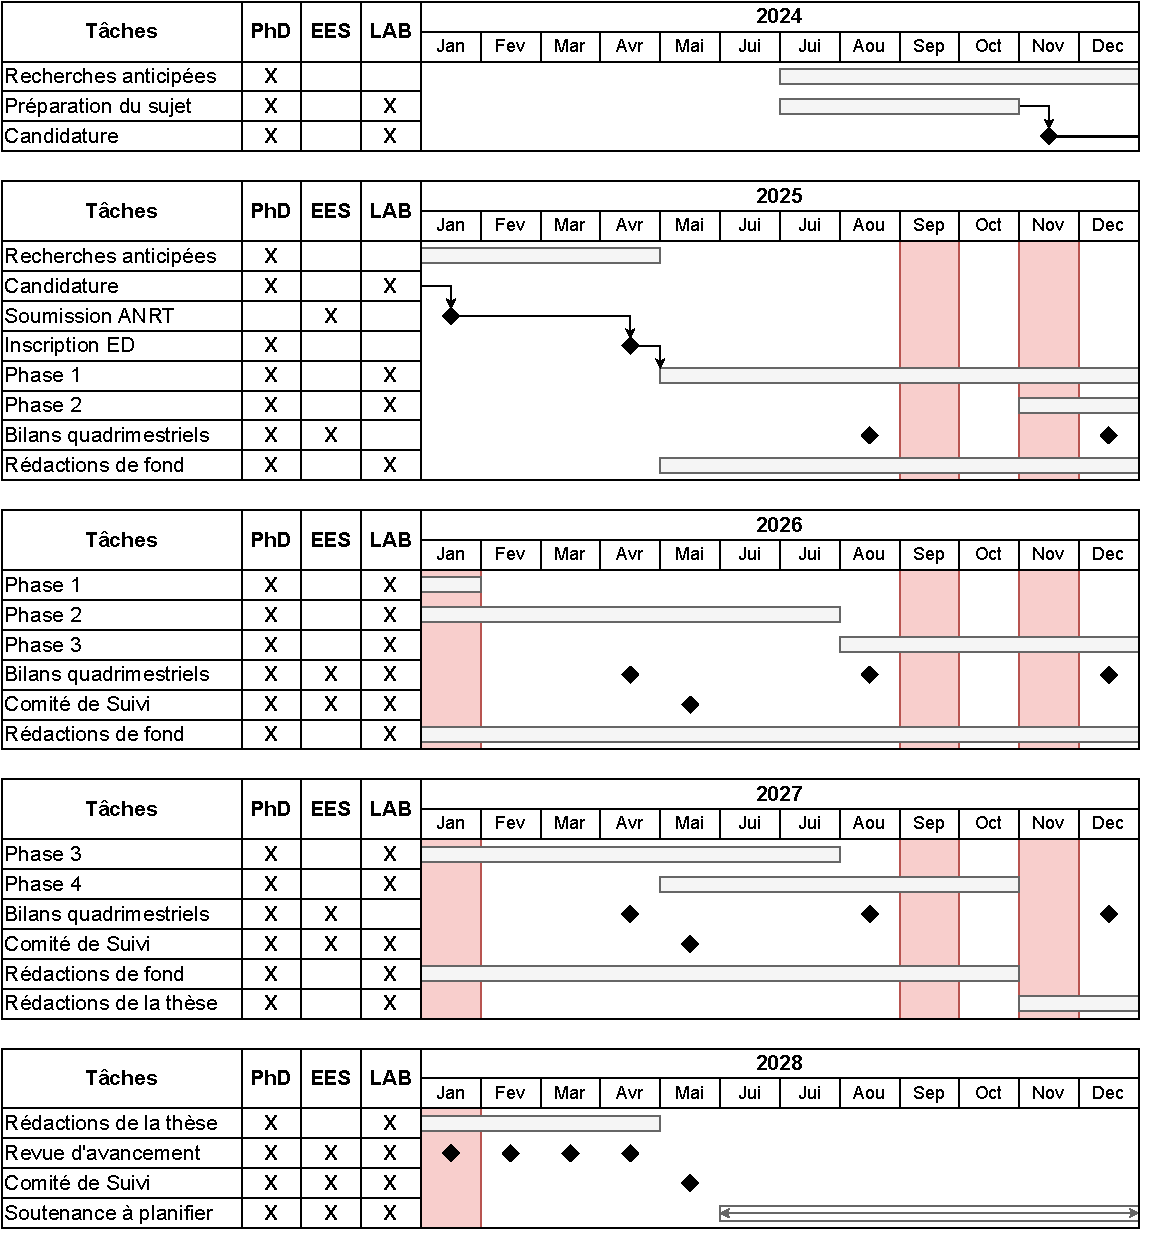
\includegraphics[width=.9\linewidth]{../svg/these-gantt-init.pdf}
\caption{\label{fig:org024fcf9}Macro-processus de traitement des contraintes durant un projet de construction avec automatisation des vérifications d’études.}
\end{figure}
\section{Modalités de suivi et d'échanges entre les partenaires}
\label{sec:org92a4dd3}
Ces modalités peuvent être vues selon plusieurs niveaux.

Pour le suivi en continu de la thèse, des échanges, qui pourront aussi bien être synchrones qu'asynchrones (visio, courriel, WhatsApp\ldots{}) se feront selon les besoins de l'activité en cours, si besoin chaque semaine, entre le doctorant (Cyprien Pierre) et les co-superviseurs côté laboratoire (Alexis Héloir et Christophe Kolski). En outre il est prévu que le doctorant passe 3 mois par an au LAMIH. Ces périodes dépendront des objectifs : réunions, formations, participation à des séminaires, campagne de tests utilisateur, etc.). Concernant les formations, 40 crédits doivent être obtenus durant la durée de la thèse, en se conformant à l'arrêté du 26 août 2022 modifiant l'arrêté du 25 mai 2016. Les modalités de formation sont visibles à :
\url{https://www.uphf.fr/recherche/lecole-doctorale/formations-doctorales/formations-doctorales-credits-cfd}

Des réunions trimestrielles seront organisées, réunissant les deux partenaires : le doctorant, les co-superviseurs côté laboratoire et Mathieu Chapel, qui est le superviseur du doctorant au sein de l'entreprise. Selon les thèmes abordés dans chaque réunion, d'autres membres du laboratoire et de l'entreprise pourront être invités.

L'évaluation de l'avancement respectera le processus basé sur un Comité de Suivi Individuel (CSI), tel que proposé par l'école doctorale et
pratiqué au LAMIH. L'avancement est évalué par le comité à la fin de chaque année de thèse. Les superviseurs (côté laboratoire et côté entreprise) sont invités à participer à ce comité. En outre, le règlement intérieur de l'ED sera respecté, en vue de l'organisation de la soutenance. Le règlement intérieur de l'école doctorale est disponible à :
\url{https://www.uphf.fr/recherche/lecole-doctorale/reglement-interieur}
\section{Moyens et matériels mis à disposition}
\label{sec:org4d9f3a2}
\begin{itemize}
\item \textbf{Côté laboratoire :} un Maître de Conférences en Informatique, co-encadrant de la thèse et un Professeur des Universités de Classe exceptionnelle 2 seront les co-superviseurs de la thèse.
\item \textbf{Côté entreprise :} Mise à disposition d'un réseau de professionnels experts, mise à disposition des corpus documentaires caractéristiques du domaine d'étude, prise en charge des frais de plateformes et d'infrastructures numériques nécessaires ainsi que de la fourniture du matériel adapté aux travaux du doctorant.
\end{itemize}
\section{Retombées attendues}
\label{sec:org968c749}
\begin{itemize}
\item \textbf{Côté laboratoire :} Les résultats attendus sont une méthode générique et une architecture de système sensible aux contraintes, ainsi que des données d'évaluation centrée utilisateur. Des publications scientifiques sont également attendues.
\item \textbf{Côté entreprise :} Les résultats attendus sont l'application de la méthode proposée sur des cas spécifiques à l'entreprise, débouchant sur un prototype de système sensible aux contraintes. Des données d'évaluation technique sont aussi attendues.
\end{itemize}
\section{Co-superviseurs de la thèse au LAMIH-UMR CNRS 8201}
\label{sec:orgddba83a}
\begin{itemize}
\item \textbf{Alexis Heloir}, Maître de Conférences en Informatique, co-encadrant de la thèse : \url{mailto:alexis.heloir@uphf.fr}
\item \textbf{Christophe Kolski}, Professeur en Informatique, directeur de la thèse : \url{mailto:Christophe.Kolski@uphf.fr}
\end{itemize}
\section{Superviseur de la thèse côté EIFFAGE ENERGIE SYSTEMES}
\label{sec:org949a322}
\begin{itemize}
\item \textbf{Mathieu Chapel}, Responsable de projet : \url{mailto:Mathieu.Chapel@eiffage.com}
\end{itemize}
\section{Références}
\label{sec:orge56c117}
\begin{multicols}{2}
\small{
\printbibliography[heading=none]
}\clearpage\end{multicols}
\section{Acronyms}
\label{sec:org060c1dd}
\textbf{\hypertarget{gls-69}{BIM}}\hspace*{1em}\hspace*{.5em}\pageref{gls-1-use-1}, \pageref{gls-1-use-2}, \pageref{gls-1-use-3}

\textbf{\hypertarget{gls-341}{VDC}}\hspace*{1em}\hspace*{.5em}\pageref{gls-2-use-1}, \pageref{gls-2-use-2}
\end{document}
